\chapter{GCN-I: Phương pháp suy diễn giá trị khuyết bằng GCN}
\label{chap:chap4}
\section{Giới thiệu}
Nhằm khắc phục vấn đề dữ liệu thưa thớt và đa dạng, khóa luận đề xuất một hướng tiếp cận hiệu quả dựa trên việc ứng dụng GCN để suy diễn và bổ sung các giá trị còn thiếu trong dữ liệu hành vi người học.

Điểm mạnh nổi bật của GCN nằm ở khả năng khai thác và mô hình hóa dữ liệu thành dạng đồ thị. Các phương pháp điền khuyết thống kê đơn giản như gán giá trị mặc định làm dữ liệu mất đi tính chất ban đầu, GCN cho phép phân tích dữ liệu trong bối cảnh toàn cục, bằng cách khai thác các kết nối giữa các thực thể trong dữ liệu. Nhờ đó, quá trình suy diễn giá trị thiếu trở nên chính xác và giàu ngữ nghĩa hơn. Điều này cho phép GCN học cách lan truyền thông tin qua các "hàng xóm" của một điểm dữ liệu khuyết, từ đó suy diễn được giá trị có ý nghĩa liên kết mật thiết với các dữ liệu xung quanh.


% Giới thiệu cách xử lý dữ liệu -> khai thác thông tin dữ liệu thế nào.
\section{Dữ liệu thực nghiệm}
\subsection{Mô tả dữ liệu}
% Trong khóa luận này, chúng tôi sử dụng bộ dữ liệu MOOCCubeX, một nguồn dữ liệu học tập quy mô lớn được thu thập từ nền tảng giáo dục trực tuyến XuetangX – một trong những nền tảng MOOC lớn nhất tại Trung Quốc. Bộ dữ liệu này cung cấp thông tin phong phú và đa dạng về hành vi học tập của người dùng, bao gồm các tương tác trên nền tảng, thời gian tham gia, thành tích học tập và đặc điểm người học. Để đảm bảo chất lượng dữ liệu và tập trung vào giai đoạn học tập mang tính quyết định, chúng tôi tiến hành tiền xử lý bằng cách lọc và tổng hợp các hành vi học tập của người dùng trong bốn tuần đầu kể từ thời điểm ghi danh, đây là giai đoạn được xem là có ảnh hưởng lớn đến khả năng hoàn thành khóa học.
% Bộ dữ liệu sau xử lý bao gồm 16.267 người học, được phân bố trên 174 khóa học khác nhau từ nhiều lĩnh vực và thuộc về 915 trường học hoặc tổ chức giáo dục.
Bộ dữ liệu \textbf{MOOCCubeX} là một nguồn tài nguyên phong phú, chứa đựng thông tin chi tiết về $4.216$ khóa học, $230.263$ video giảng dạy, $358.265$ bài tập, và $637.572$ khái niệm chi tiết (fine-grained) \cite{yu2021mooccubex}. Đặc biệt, bộ dữ liệu này ghi nhận hơn $296$ triệu bản ghi thô về hành vi của người học, với sự tham gia của $3.330.294$ sinh viên. MOOCCubeX được cấu trúc thành hai phần chính: \textbf{Tài nguyên khóa học (Course resources)} và \textbf{Hành vi người học (Student behavior)}.
Phần \textit{Course resources} trình bày chi tiết về các loại tài nguyên học tập được tích hợp trong mỗi khóa học, bao gồm:

\begin{itemize}
    \item \textbf{Thông tin khóa học:} Tên khóa học, giáo viên, trường học cung cấp, mã khóa học, lĩnh vực, và độ dài khóa học.
    \item \textbf{Nội dung học tập:} Danh sách các tài nguyên như video bài học, bài tập, và đề thi.
    \item \textbf{Thời gian và tiến trình học:} Ghi lại các mốc thời gian khóa học bắt đầu và kết thúc cũng như các yêu cầu về tiến trình học.
    \item \textbf{Cấu trúc khóa học:} Sự phân chia thành các phần hoặc tuần học, số lượng bài giảng và bài tập yêu cầu.
\end{itemize}
Thông tin trong \textit{Course resources} phản ánh cụ thể khối lượng và nội dung học tập mà người học cần hoàn thành trong từng khóa học. 

\textit{Student behaviors} là tập dữ liệu ghi lại thông tin người học và các hành vi học tập trên nền tảng XuetangX, bao gồm:
\begin{itemize}
    \item \textbf{Thông tin người học:} Bao gồm tên người dùng, mã người dùng, giới tính, trường học.
    \item \textbf{Hoạt động xem video:} Tổng thời gian xem video, tần suất truy cập các bài giảng video trong từng khóa học.
    \item \textbf{Tham gia diễn đàn thảo luận:} Số lượng bài viết, bình luận, và trả lời của sinh viên trong các diễn đàn khóa học.
    \item \textbf{Làm bài tập và bài kiểm tra:} Ghi nhận các nỗ lực làm bài tập, bài kiểm tra và điểm số đạt được.
    \item \textbf{Tương tác trên Xiaomu:} Sự tương tác của người học với Xiaomu (QA bot của XueTangX).
\end{itemize}
Dữ liệu từ \textit{Student behaviors} thể hiện rõ cách sinh viên tương tác với các khóa học, qua đó hỗ trợ việc nhận diện các hành vi học tập mang tính tích cực hoặc tiêu cực. Khi kết hợp với dữ liệu \textit{Course resources}, chúng tạo thành một cái nhìn tổng thể, vừa bao quát nội dung học tập vừa phản ánh phương thức tiếp cận của người học.


% Mô tả chi tiết của các bảng dữ liệu trong bộ dữ liệu MOOCCubeX sẽ được trình bày trong các mục tiếp theo.

\subsection{Phân tích dữ liệu}
Trong khuôn khổ khóa luận, bộ dữ liệu được xây dựng bằng việc tổng hợp, xử lý và hợp nhất từ nhiều tệp dữ liệu riêng biệt:
\begin{itemize}
    \item \texttt{entities/user.json}: Thông tin người học (user).
    \item \texttt{relations/user-problem.json}: Tương tác người học với bài tập.
    \item \texttt{relations/user-video.json}: Tương tác người học với video bài giảng.
    \item \texttt{entities/reply.json}: Dữ liệu phản hồi trên diễn đàn.
    \item \texttt{entities/comment.json}: Dữ liệu bình luận trên diễn đàn.
\end{itemize}

 Bộ dữ liệu thu được có cấu trúc bảng duy nhất, với mỗi dòng đại diện cho một người học trong một khóa học cụ thể, bao gồm: 16,267 entries (dòng) và 16 columns (cột). Sau đây chúng tôi sẽ tóm tắt các cột của bộ dữ liệu qua bảng sau:
\begin{table}[H]
\centering
\caption{Mô tả thuộc tính trong tập dữ liệu}
\label{tab:dataset_description}
\begin{tabular}{|c|l|p{7cm}|c|}
\hline
\textbf{STT} & \textbf{Thuộc tính} & \textbf{Mô tả} & \textbf{Kiểu dữ liệu} \\ \hline
1  & user\_id            & Mã định danh cho mỗi người học                                 & Object \\ \hline
2  & course\_id          & Mã định danh cho mỗi khóa học                                 & Object \\ \hline
3  & gender              & Giới tính                                                    & Float  \\ \hline
4  & year\_of\_birth      & Năm sinh người học                                           & Float  \\ \hline
5  & school              & Tên trường mỗi người dùng                                    & Object \\ \hline
6  & teacher\_name       & Tên giáo viên của mỗi khóa học                               & Object \\ \hline
7  & enroll\_time        & Thời gian người dùng đăng ký khóa học                       & Object \\ \hline
8  & last\_submit\_time   & Thời gian nộp bài tập cuối cùng                              & Object \\ \hline
9  & comment\_count      & Số lượng bình luận của người học tương tác trên diễn đàn thảo luận   & Float  \\ \hline
10 & reply\_count        & Số lượng các câu hồi đáp trên diễn đàn thảo luận            & Float  \\ \hline
11 & user\_watching\_time & Thời gian người dùng xem các video bài học                  & Float  \\ \hline
12 & total\_score        & Tổng điểm bài tập của người dùng                             & Float  \\ \hline
13 & assignment\_count   & Tổng số các bài tập của người dùng                           & Int    \\ \hline
14 & total\_attempts     & Tổng số lần nộp bài của người dùng                           & Int    \\ \hline
15 & final\_exam\_score   & Điểm bài tập cuối kỳ                                         & Float  \\ \hline
16 & duration\_days      & Thời gian người dùng tham gia khóa học                      & Float  \\ \hline
% 17 & classification      & Xếp loại học tập người dùng cuối cùng                        & Object \\ \hline
\end{tabular}
\end{table}

\begin{figure}[H]
    \centering
    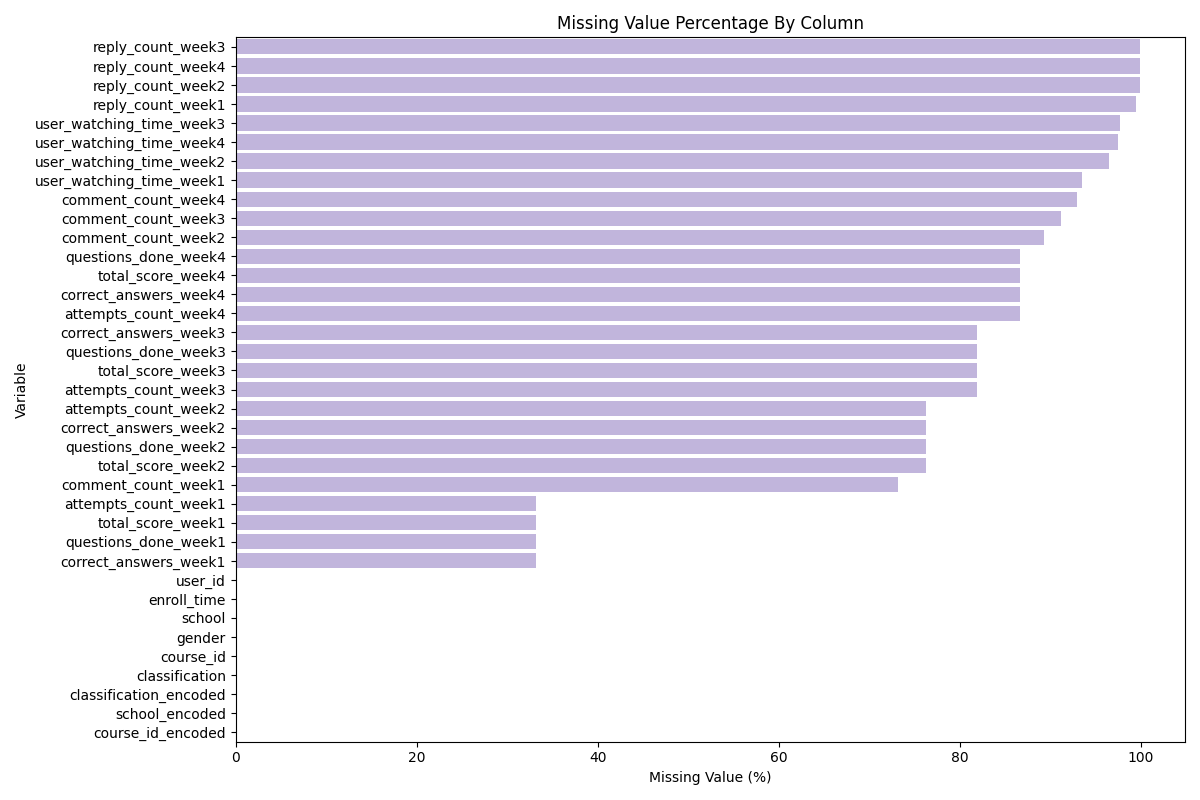
\includegraphics[width=0.9\textwidth]{imgs/missing-values-chart.png}
    \caption{Đặc điểm phân bố của dữ liệu thiếu trên các thuộc tính}
    \label{fig:percentage of missing values}
\end{figure}


 Trong \textbf{Hình \ref{fig:percentage of missing values}}, chúng ta có thể thấy được tình trạng đầy đủ của các trường dữ liệu. Đặc biệt, các thuộc tính liên quan đến hành vi học tập theo từng tuần như: \textit{reply\_count\_week3}, \textit{comment\_count\_week3}, \textit{attempts\_count\_week3} hay \textit{correct\_answer\_week3} đều có mức độ khuyết dữ liệu nghiêm trọng. Ngược lại, các cột định danh như \textit{user\_id}, \textit{course\_id}, cùng với một số thông tin đăng ký như \textit{enroll\_time}, lại có tỷ lệ thiếu không đáng kể hoặc gần như đầy đủ.

Tình trạng này gây ra trở ngại cho việc xây dựng mô hình dự đoán đáng kể do tính chất dữ liệu thiếu và không đồng nhất.


% \textbf{Hình \ref{fig:Histogram of Classification}} là biểu đồ tần suất của biến classification cho thấy sự phân bố không đồng đều giữa các nhóm xếp loại học tập. Trong đó, nhóm E chiếm tỷ lệ lớn nhất, vượt xa so với các nhóm còn lại với hơn 14.000 mẫu. Nhóm A xếp thứ hai với khoảng 6.000 mẫu, trong khi các nhóm B, C và D có số lượng tương đối thấp và khá cân bằng, dao động từ 1.000 đến 2.000 mẫu.

% Sự chênh lệch này phản ánh tính mất cân bằng nhãn (label imbalance) rõ rệt trong tập dữ liệu, đây là một yếu tố quan trọng cần được xem xét trong quá trình huấn luyện mô hình. Việc mất cân bằng có thể khiến mô hình nghiêng về việc dự đoán các lớp chiếm ưu thế như E và A, từ đó làm giảm độ chính xác đối với các lớp hiếm. Do đó, trong các bước tiếp theo, cần cân nhắc sử dụng các kỹ thuật xử lý mất cân bằng dữ liệu như oversampling, undersampling hoặc gán trọng số lớp để đảm bảo mô hình học được đầy đủ từ mọi phân lớp.

\begin{figure}[H]
    \centering
    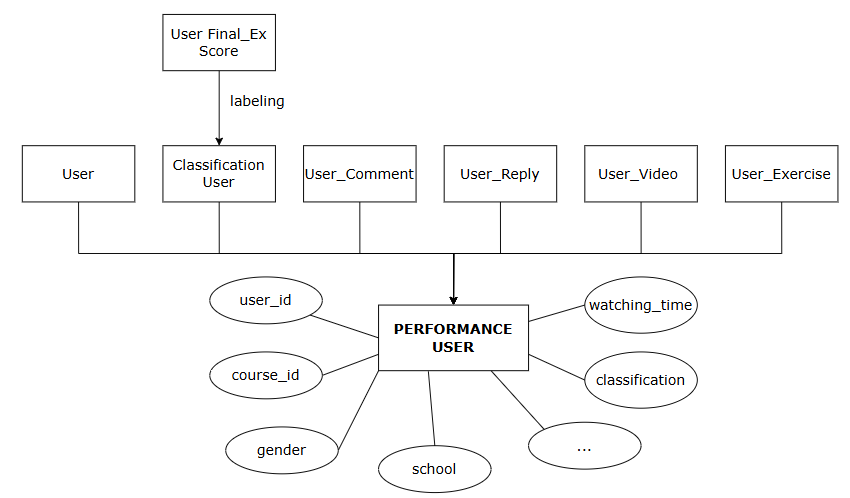
\includegraphics[width=0.9\textwidth]{imgs/data-transform.png}
    \caption{Quy trình chuyển đổi dữ liệu}
    \label{fig:data-transform}
\end{figure}

Sơ đồ tổng quan về quy trình chuyển đổi được minh họa trong Hình~\ref{fig:data-transform} cho chúng ta nắm bắt phương pháp chúng tôi hợp nhất các file dữ liệu.
Quá trình này bắt đầu từ thực thể \textbf{User}, đại diện cho người học trong nền tảng MOOC. Dữ liệu từ người dùng được liên kết với các nguồn dữ liệu phụ như:

\begin{itemize}
    \item \textbf{Classification User}: thông tin xếp loại người học dựa trên điểm số cuối kỳ.
    \item \textbf{User\_Comments} và \textbf{User\_Reply}: dữ liệu hành vi người dùng trên diễn đàn thảo luận (số lượng bình luận, trả lời).
    \item \textbf{User\_Video}: thông tin thời lượng người học xem video bài giảng.
    \item \textbf{User\_Exercise}: các tương tác của người dùng với bài tập (số lần nộp bài, số điểm đạt được, số câu đúng, \ldots).
\end{itemize}

Tất cả các nguồn dữ liệu phụ trên được liên kết trở lại với người học thông qua thực thể trung tâm \textbf{Performance User}, chứa các đặc trưng như:

\begin{itemize}
    \item \textbf{Thông tin cá nhân}: \textit{gender}, \textit{year\_of\_birth}, \textit{school}.
    \item \textbf{Thông tin hoạt động}: \textit{comment\_count}, \textit{reply\_count}, \textit{watching\_time}, \textit{assignment\_count}, \textit{final\_exam\_score}, \textit{v.v}.
\end{itemize}

Các tập dữ liệu rời rạc được liên kết với nhau thông qua các khóa định danh chính như \textit{user\_id} và \textit{course\_id}. Việc tổ chức dữ liệu theo cấu trúc Performance User đóng vai trò trung tâm. Thông qua quá trình tích hợp và chuẩn hóa theo chiều dọc dựa trên các khóa chính, dữ liệu được gom lại sao cho mỗi dòng trong bảng tổng hợp cuối cùng đại diện cho một cá nhân cụ thể, với đầy đủ các đặc trưng cần thiết cho mô hình dự đoán. 

\subsection{Chiến lược gán nhãn và chuẩn hóa thang điểm}
Dữ liệu từ nền tảng MOOCCubeX bao gồm hàng trăm khóa học đến từ nhiều quốc gia và tổ chức giáo dục khác nhau, với mỗi đơn vị áp dụng một hệ thống thang điểm riêng biệt (chẳng hạn: thang 10, thang 20, thang 4.0 của Mỹ, thang 6 của Đức, v.v.). Sự đa dạng này tạo ra thách thức trong việc chuẩn hóa để phục vụ cho quá trình quá trình dự đoán. Do đó, chúng tôi đã thực hiện một khảo sát các thang điểm hiện hành trên thế giới, giúp quá trình gán nhãn trở nên chính xác và đáng tin cậy hơn.

\subsubsection{Khảo sát thang điểm quốc tế}
Tổng cộng, nhóm đã khảo sát 73 hệ thống thang điểm khác nhau về: 
\begin{itemize}
    \item Loại thang điểm sử dụng (thang điểm 10, 20, 4.0, 6, 100, \ldots)
    \item Số lượng khóa học áp dụng mỗi loại thang điểm
    \item Sự tồn tại hay không của mô tả phân loại kết quả học tập
    \item Phân loại học lực tương ứng với các mức độ như: Xuất sắc, Giỏi, Khá, Trung bình, Yếu và Kém.
\end{itemize}

Trong đó, tôi tập trung vào 13 thang điểm phổ biến có đủ thông tin phân loại, như:

\begin{itemize}
    \item Thang 10 điểm (159 khóa học): 
    \textit{Phổ biến tại Việt Nam}
    
    \item Thang 5 điểm (106 khóa):
    \textit{Áp dụng rộng rãi tại Nga}

    \item Thang 20 điểm (87 khóa):
    \textit{Thường dùng ở Pháp}

    \item Thang 6 điểm (77 khóa):
    \textit{Theo hệ thống giáo dục Đức}

    \item Thang 4.0 (65 khóa):
    \textit{Một số đại học quốc tế sử dụng}
\end{itemize}


\subsubsection{Chiến lược chuẩn hóa về 5 mức độ của Coursera}

Sau quá trình khảo cứu nhiều hệ thống phân loại học lực từ các quốc gia và nền tảng đào tạo trực tuyến khác nhau, chúng tôi quyết định chuẩn hóa toàn bộ dữ liệu điểm số về \textbf{thang 5 mức độ} được sử dụng bởi nền tảng \textit{Coursera}, một trong những hệ thống MOOC lớn và có sức ảnh hưởng toàn cầu.

Việc lựa chọn thang điểm này không chỉ dựa trên tính phổ biến, mà còn bởi nó có cấu trúc rõ ràng, dễ hiểu, với các mức đánh giá cụ thể từ ``Xuất sắc'' đến ``Chưa hoàn thành''. Điều này đặc biệt quan trọng trong bối cảnh dữ liệu MOOCCubeX sử dụng nhiều thang điểm khác nhau do sự khác biệt của mỗi quốc gia, ví dụ thang điểm 10, thang điểm 20, GPA 4.0 hoặc thang điểm 6 của Đức. Thang điểm của Coursera giúp tạo nên một chuẩn chung, cho phép quy đổi linh hoạt và \textbf{giảm thiểu sai lệch do sự không đồng nhất trong hệ thống đánh giá ban đầu}.

Hơn nữa, hệ thống phân loại này được thiết kế với sự cân bằng giữa tính chi tiết và tính tổng quát, vừa phản ánh được năng lực học tập thực tế của người học, vừa phù hợp để tích hợp vào các mô hình học máy, nơi cần các nhãn nhất quán và dễ diễn giải. Việc sử dụng thang điểm 5 mức từ Coursera cũng giúp nâng cao \textbf{tính khả chuyển của kết quả mô hình}, đồng thời hỗ trợ dễ dàng hơn cho các phân tích so sánh liên quốc gia hoặc giữa các tổ chức giáo dục khác nhau.



\vspace{0.5em}
\begin{table}[H]
\centering
\caption{Chiến lược chuẩn hóa điểm số về thang điểm Coursera}
\label{tab:coursera_grading}
\renewcommand{\arraystretch}{1.6} 
\begin{tabular}{|c|>{\centering\arraybackslash}p{7cm}|>{\centering\arraybackslash}p{2.5cm}|}
\hline
\textbf{Mức độ} & \textbf{Mô tả} & \textbf{Nhãn gán} \\
\hline
Distinction & 85–100\% -- Xuất sắc, thành tích vượt trội & A \\
\hline
Merit & 70–84\% -- Giỏi, kiến thức vững & B \\
\hline
Pass & 50–69\% -- Đạt yêu cầu tối thiểu & C \\
\hline
Fail & Dưới 50\% -- Không đạt yêu cầu & D \\
\hline
Incomplete & Không làm bài thi cuối kỳ hoặc bỏ dở & E \\
\hline
\end{tabular}
\end{table}
\vspace{0.5em}

Việc gán nhãn này được thực hiện cho từng học viên trong mỗi khóa học, dựa trên thang điểm cụ thể mà khóa học đó sử dụng. Các quy tắc chuyển đổi được tham khảo từ tài liệu chính thức của từng quốc gia hoặc nền tảng MOOC, và được mã hóa thành logic tự động trong pipeline xử lý dữ liệu của hệ thống.
\noindent Dựa trên nguyên tắc trên, tôi đã tiến hành chuyển đổi các hệ thống thang điểm hiện có thành nhãn đầu ra phục vụ cho mô hình học sâu. Bảng dưới đây trình bày một số ví dụ điển hình của các hệ thống thang điểm có chiến lược gán nhãn rõ ràng:

\begin{table}[H]
\centering
\caption{Tổng hợp các hệ thống thang điểm và chiến lược gán nhãn}
\begin{tabular}{|c|p{2.5cm}|p{2.8cm}|p{6cm}|}
\hline
\textbf{STT} & \textbf{Thang điểm} & \textbf{Phân loại gốc} & \textbf{Chiến lược gán nhãn (theo Coursera)} \\
\hline
1 & 10 (Việt Nam) & Xuất sắc: 9-10; Giỏi: 8-<9; Khá: 7-<8; Trung bình: 5-<7; Yếu: 4-<5; Kém: <4 & 
A: 9-10 \newline
B: 8-<9 \newline
B: 7-<8 \newline
C: 5-<7 \newline
D: <5 \newline
E: Không thi cuối kỳ \\
\hline
2 & 5 (Nga) & Excellent (5), Good (4), Satisfactory (3), Unsatisfactory (2) & 
A: 5 \newline
B: 4 \newline
C: 3 \newline
D: 2 \newline
E: Không thi cuối kỳ \\
\hline
3 & 20 (Pháp) & Xuất sắc: 18-20; Giỏi: 16-<18; Khá: 14-<16; Trung bình: 10-<14; Kém: <10 & 
A: 18-20 \newline
B: 16-<18 \newline
B: 14-<16 \newline
C: 10-<14 \newline
D: <10 \newline
E: Không thi cuối kỳ \\
\hline
4 & 6 (Đức) & 1 (Very Good) đến 6 (Inadequate) & 
A: 1 \newline
B: 2 \newline
C: 3-4 \newline
D: 5-6 \newline
E: Không thi cuối kỳ \\
\hline
5 & 100 (Mỹ) & Xuất sắc: 90-100; Giỏi: 80-89; Khá: 70-79; Trung bình khá: 60-69; Trung bình: 50-59; Kém: <50 & 
A: 90-100 \newline
B: 80-89 \newline
B: 70-79 \newline
C: 50-69 \newline
D: <50 \newline
E: Không thi cuối kỳ \\
\hline
\end{tabular}
\label{tab:grading_conversion}
\end{table}

Kết quả cho thấy việc quy đổi điểm số về thang 5 mức không chỉ tạo ra một thuộc tính chung, mà còn giúp cải thiện hiệu quả huấn luyện.

 
% Để xây dựng hệ thống khuyến nghị khóa học, khoá luận đã thực hiện các thí nghiệm sử dụng dữ liệu từ bộ dữ liệu MOOCCubeX của nền tảng MOOC XuetangX tại Trung Quốc. Bộ dữ liệu này bao gồm thông tin về người dùng, các khóa học họ đã đăng ký, và các danh mục khóa học tương ứng (tham khảo Bảng \ref{tab:right} để biết thêm chi tiết).
% Với dữ liệu khoá học được mô tả trong bảng \ref{tab:course_info}, em em có các thuộc tính như sau:
Sau đó, chúng tôi tiến hành tiền xử lý bằng cách lọc và tổng hợp các hành vi học tập của người dùng trong bốn tuần đầu kể từ thời điểm ghi danh, đây là giai đoạn được xem là có ảnh hưởng lớn đến khả năng hoàn thành khóa học.
Bộ dữ liệu sau xử lý bao gồm 16.267 người học, được phân bố trên 174 khóa học khác nhau từ nhiều lĩnh vực và thuộc về 915 trường học hoặc tổ chức giáo dục. Dựa trên chiến lược gán nhãn và chuẩn hóa thang điểm đã đề cập, kết quả hoàn thành khóa học cuối cùng của người học được chia thành năm nhóm theo mức độ hoàn thành chuẩn đầu ra, bao gồm: A (Xuất sắc), B (Tốt), C (Đạt yêu cầu), D (Chưa đạt) và E (Không hoàn thành khóa học).
\begin{figure}[H]
    \centering
    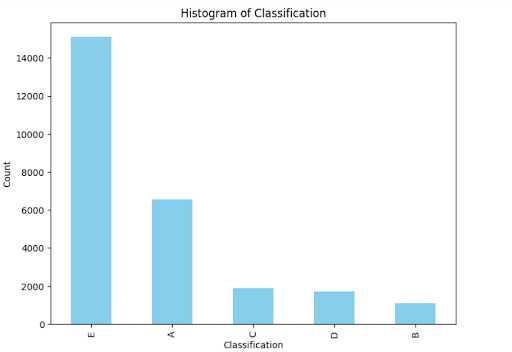
\includegraphics[width=0.9\textwidth]{imgs/Histogram of Classification.png}
    \caption{Biểu đồ phân phối nhãn học lực sau chuẩn hóa}
    \label{fig:label}
\end{figure}

Hình  \ref{fig:label} phản ánh sự mất cân bằng dữ liệu: nhóm E (Không hoàn thành) chiếm phần lớn với 61,14\%, theo sau là nhóm A (Xuất sắc) với 22,88\%. Trong khi đó, các nhóm còn lại lần lượt là B (3,37\%), C (6,34\%), và D (6,27\%), là các nhóm thể hiện hiệu suất trung bình hoặc yếu nhưng chiếm tỷ lệ thấp hơn nhiều. 
\begin{table*}[htbp]
\caption{Tổng quan bộ dữ liệu và phân bố nhãn}
\label{tab:combined-tables}
\centering
\begin{minipage}[t]{0.65\textwidth} % mở rộng bảng mô tả
\centering
\small % giảm cỡ chữ bảng mô tả
\renewcommand{\arraystretch}{1.3}
\textbf{(a) Mô tả bộ dữ liệu}
\vspace{2mm}

\begin{tabularx}{\textwidth}{|>{\raggedright\arraybackslash}p{3.4cm}|>{\centering\arraybackslash}m{1.2cm}|>{\raggedright\arraybackslash}X|}
\hline
\textbf{Đặc trưng} & \textbf{Loại dữ liệu} & \textbf{Mô tả} \\
\hline
User & Object & Người dùng đã đăng ký khóa học \\
Course & Object & Khóa học mà người học đăng ký \\
School & Object & Trường mà người học theo học \\
Gender & Integer & Giới tính của người học \\
Enroll\_time & Datetime & Thời điểm đăng ký khóa học \\
comment\_count\_week \textit{i} & Float & Số lượng bình luận trong tuần \textit{i} \\
reply\_count\_week \textit{i} & Float & Số lượng phản hồi trong tuần \textit{i} \\
questions\_done\_week \textit{i} & Float & Số lượng câu hỏi đã làm trong tuần \textit{i} \\
attempts\_count\_week \textit{i} & Float & Số lần làm bài kiểm tra trong tuần \textit{i} \\
correct\_answers\_week \textit{i} & Float & Số lượng câu trả lời đúng trong tuần \textit{i} \\
total\_score\_week \textit{i} & Float & Tổng điểm bài kiểm tra trong tuần \textit{i} \\
user\_watching\_time\_week \textit{i} & Float & Tổng thời lượng xem video (giờ) trong tuần \textit{i} \\
classification & Object & Nhãn kết quả hoàn thành khóa học cuối cùng \\
\hline
\multicolumn{3}{l}{$^{\mathrm{*}}$\textit{i} đại diện cho tuần 1 - 4.}
\end{tabularx}
\end{minipage}
\hfill
\begin{minipage}[t]{0.32\textwidth} % thu hẹp bảng phân phối
\centering
\small % giảm cỡ chữ bảng label
\renewcommand{\arraystretch}{1.3}
\textbf{(b) Tỷ lệ phân bố nhãn}
\vspace{2mm}

\begin{tabular}{|c|c|c|}
\hline
\textbf{Nhãn} & \textbf{Số lượng} & \textbf{Tỷ lệ} \\
\hline
A  & 3,722 & 22.88\% \\
B  & 548 & 3.37\% \\
C  & 1,032 & 6.34\% \\
D  & 1,020 & 6.27\% \\
E  & 9,945 & 61.14\% \\
\hline
\textbf{Tổng} & 16,267 & 100.00\% \\
\hline
\end{tabular}
\end{minipage}
\end{table*}
Sự chênh lệch đáng kể này tạo ra một bài toán mất cân bằng lớp (class imbalance), khi mô hình học máy thường có xu hướng thiên lệch về các lớp có tần suất xuất hiện cao hơn, dẫn đến tình trang học hỏi kém hiệu quả với những lớp nhãn ít xuất hiện.

Đây chính là vấn đề chúng ta thường gặp khi giải quyết các bài toán phân loại. Nhằm bảo vệ dữ liệu có tần suất xuất hiện thấp (như nhóm D (không đạt)), chúng ta có những phương pháp tăng mẫu dữ liệu, điển hình là phương pháp tổng hợp mẫu thiểu số SMOTE. Mục tiêu chính là nâng cao khả năng nhận biết của mô hình đối với các nhóm dữ liệu thiểu số.
% ------
\section{Phương pháp đề xuất}
Mục tiêu của phần này là làm rõ cách mô hình hoạt động và quy trình GCN-I thực hiện suy diễn giá trị thiếu, tất cả nhằm hướng đến việc cải thiện chất lượng của bộ dữ liệu đầu vào.

\begin{figure}[t]
    \centering
    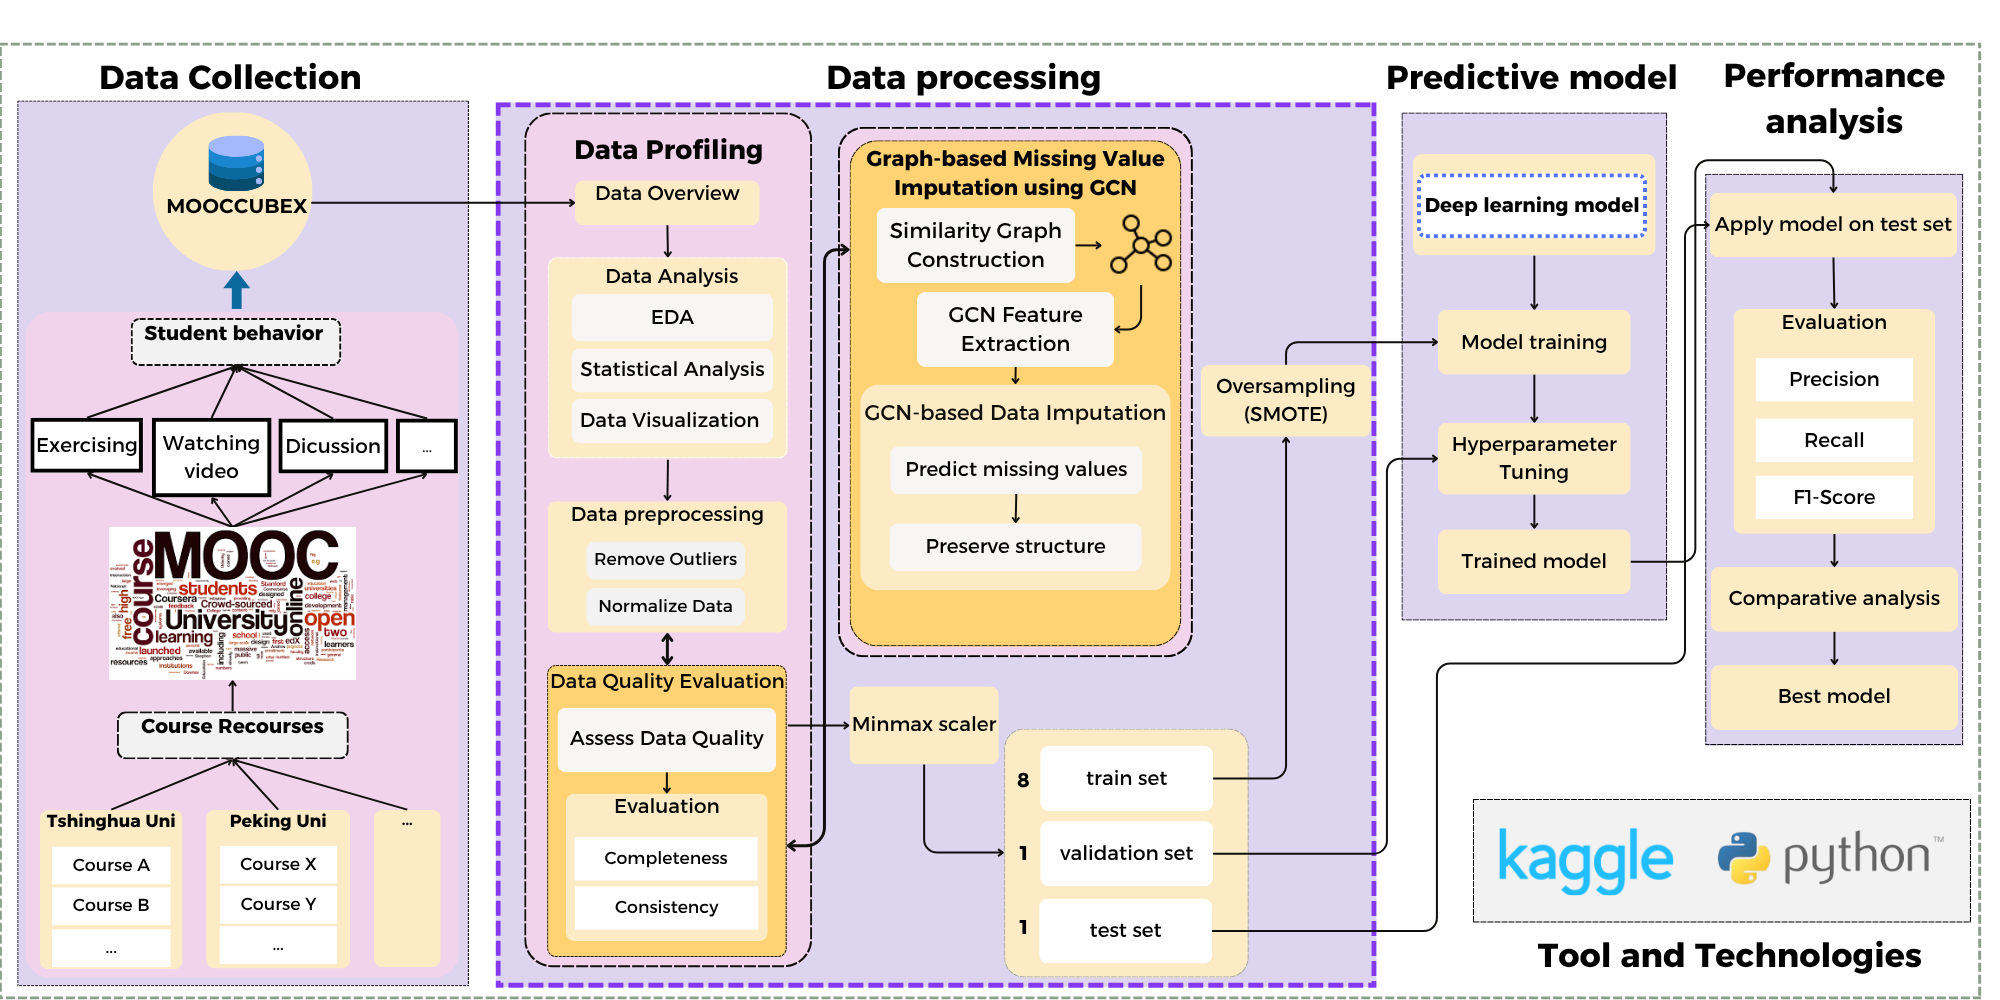
\includegraphics[width = \textwidth]{imgs/system-logo.png}
    \caption{Flowchart thể hiện quy trình hệ thống}
    \label{fig:System-img}
\end{figure}
  Quy trình xử lý dữ liệu tổng thể của nghiên cứu được thể hiện qua sơ đồ ở \textbf{Hình \ref{fig:System-img}}. Toàn bộ kiến trúc được cấu thành từ bốn bước chính: thu thập dữ liệu, tiền xử lý, huấn luyện mô hình và phân tích kết quả. 

Đầu tiên là thu thập dữ liệu từ các nền tảng MOOCs, gồm thông tin về sinh viên cùng với thông tin khóa học. Sau bước thu thập, dữ liệu được đưa vào quy trình tiền xử lý  bao gồm bốn bước chính: Data Overview, Data Analysis, Data Preprocessing và Data Quality Evaluation. Tổng thể của dữ liệu được nắm bắt thông qua các kiểm tra kích thước, loại thuộc tính và tỷ lệ thiếu giá trị. Chúng tôi thể hiện các xu hướng phân phối dữ liệu hoặc mối quan hệ giữa các biến bằng biểu đồ trực quan hóa và thống kê mô tả. Tiếp theo, việc đánh giá chất lượng dữ liệu được thực hiện để xác định tình trạng hiện tại của dữ liệu, từ đó đưa ra các quyết định điều chỉnh phù hợp. Những điểm dữ liệu cực đoan có khả năng gây nhiễu quá trình huấn luyện, thông qua phương pháp khoảng tứ phân vị (IQR) kết hợp với biểu đồ hộp (Box Plot), chúng ta tiến hành loại bỏ. 

Khác với các quy trình truyền thống chỉ thực hiện một vòng xử lý, chúng tôi tiến hành đánh giá chất lượng dữ liệu nhiều lần, đặc biệt là sau khi hoàn tất các bước xử lý sơ bộ. Mục tiêu là kiểm tra mức độ cải thiện đạt được, từ đó đảm bảo tập dữ liệu đã sẵn sàng cho giai đoạn suy diễn giá trị thiếu bằng phương pháp GCN mà nghiên cứu đề xuất.


GCN-I được chúng tôi áp dụng để suy diễn giá trị khuyết của tập dữ liệu, trong đó các nút biểu diễn người học và các cạnh đại diện cho các thuộc tính chung như trường học, khóa học đã đăng ký hoặc sự tương đồng dữ liệu. Nếu mật độ cạnh quá thấp, chúng tôi sẽ thêm các cạnh bổ sung dựa trên các chỉ số tương đồng. Cơ chế bổ sung giá trị được xây dựng trên kiến trúc hai giai đoạn Generator–Discriminator như \textbf{Hình \ref{fig:GCN-Imputer}}. Khác với GCN truyền thống, kiến trúc này nâng cao độ chính xác khi bổ sung giá trị thiếu thông qua học đối kháng, cho phép bộ sinh (generator) liên tục cải thiện các giá trị khuyết dựa trên phản hồi từ bộ phân biệt (discriminator). Chúng tôi áp dụng chỉ số sai số bình phương trung bình (MSE) giữa các giá trị thực và giá trị được bổ sung để đánh giá chất lượng của quá trình điền khuyết. Sau khi hoàn thành quá trình, quá trình đánh giá chất lượng được thực hiện lại theo các độ đo chất lượng trực tiếp và gián tiếp, giúp theo dõi chặt chẽ sự cải thiện và đảm bảo dữ liệu đầu vào sạch, tối ưu cho các bước học máy tiếp theo.

Sau khi hoàn tất quá trình bổ sung giá trị thiếu bằng phương pháp GCN, dữ liệu được tiếp tục xử lý bằng  MinMax Scaler nhằm đưa các đặc trưng về cùng một khoảng giá trị chuẩn. Tập dữ liệu sau đó được phân chia thành ba phần theo tỷ lệ 8:1:1, tương ứng với các tập Train, Validation và Test.

Một trong những thách thức ban đầu được ghi nhận là tình trạng mất cân bằng lớp (class imbalance) trong tập dữ liệu. Để giải quyết vấn đề này và đảm bảo mô hình không bị thiên vị về phía các lớp đa số, chúng tôi đã áp dụng kỹ thuật lấy mẫu vượt trội cho lớp thiểu số tổng hợp, hay còn gọi là SMOTE (Synthetic Minority Over-sampling Technique). Kỹ thuật này giúp cân bằng lại sự phân bố của các nhãn, qua đó tăng cường khả năng nhận diện của mô hình đối với các nhóm thiểu số.

Khi chuẩn bị xong dữ liệu, quá trình huấn luyện mô hình học sâu được bắt đầu, bao gồm: 4-layer Stacked LSTM, GRU, RNN và BiLSTM. Để có một sự so sánh khách quan và toàn diện, hiệu năng của mỗi mô hình được định lượng thông qua một bộ các chỉ số đánh giá đa dạng. Mô hình thể hiện hiệu suất tốt nhất qua các bài kiểm tra này sẽ được lựa chọn để tích hợp làm nhân xử lý chính cho hệ thống website dự đoán kết quả hoàn thành khóa học.
\subsubsection{Kiến trúc GCN-Imputer}

\begin{figure}[t]
    \centering
    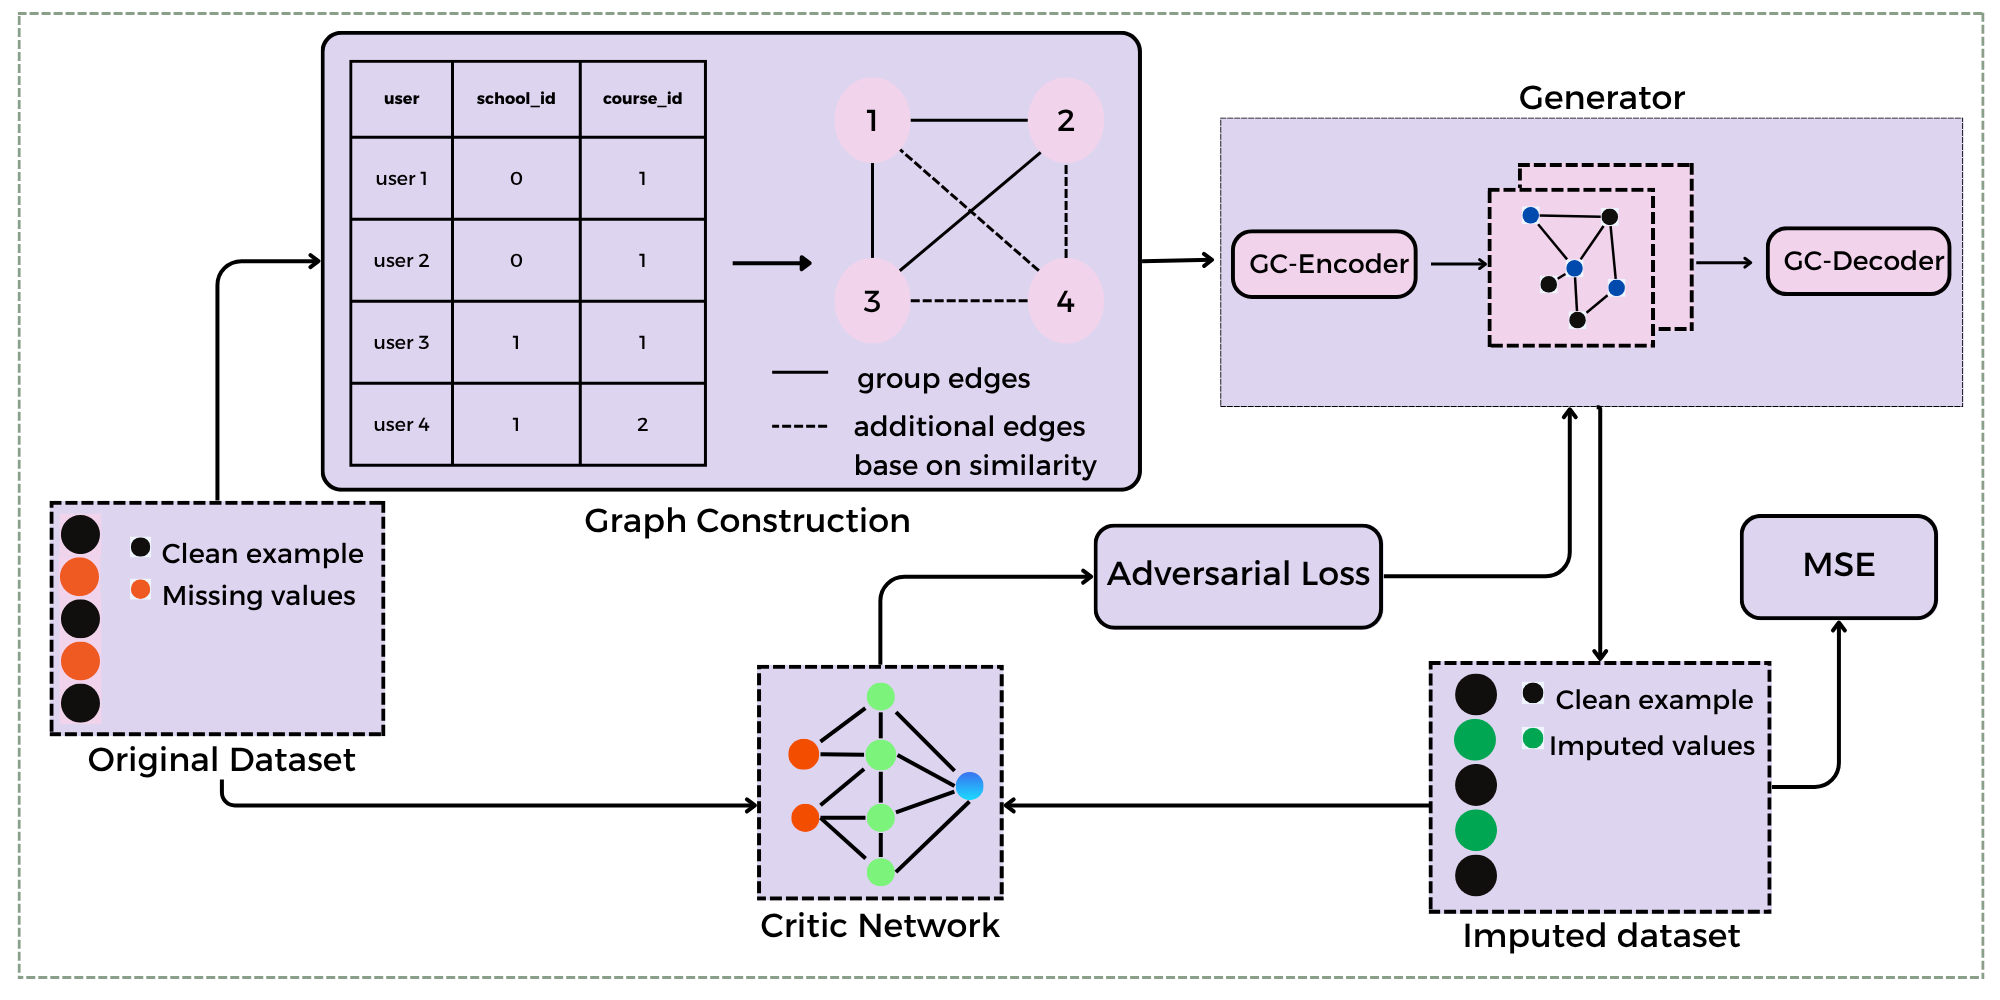
\includegraphics[width = \textwidth]{imgs/gcn-newtone.png}
    \caption{Kiến trúc mô hình GCN-Imputer}
    \label{fig:GCN-Imputer}
\end{figure}
Mô hình GCN-Imputer được thể hiện ở (\textbf{Hình \ref{fig:GCN-Imputer}}), một phương pháp hoàn thiện dữ liệu dựa trên GCN, kết hợp với mô hình sinh–phân biệt (Generator–Discriminator). Kiến trúc này không chỉ tận dụng được thông tin cấu trúc từ dữ liệu gốc thông qua xây dựng đồ thị, mà còn nâng cao độ chính xác của giá trị được điền bằng cách học sinh dữ liệu và phân biệt theo hướng đối kháng (adversarial learning). 

\textbf{Biểu diễn dữ liệu dưới dạng đồ thị (Graph Construction):} Thay vì xử lý dữ liệu theo dạng bảng truyền thống, phương pháp này bắt đầu bằng việc chuyển đổi dữ liệu ban đầu thành một ma trận đặc trưng, và xây dựng các thể (người học) là các đỉnh của đồ thị. Chúng tôi xác định sự tương đồng về đặc trưng hoặc mối quan hệ nhóm để xây dựng các liên kết (cạnh). Bằng cách biểu diễn dữ liệu như vậy, các thông tin về cấu trúc và những liên kết tiềm ẩn giữa các bản ghi có thể được làm rõ.

\vspace{0.5em}

\textbf{Bộ sinh (Generator):} Generator bao gồm một encoder và một decoder sử dụng GCN. Bộ encoder học biểu diễn đặc trưng dữ liệu có khuyết thiếu, trong khi decoder sử dụng các đặc trưng đó để ước lượng và điền vào các giá trị còn thiếu. Đây là bước học sinh tích cực nhằm tái tạo dữ liệu đầy đủ.

\vspace{0.5em}

\textbf{Bộ phân biệt (Critic/Discriminator):} Bộ Critic đóng vai trò như một mạng nơ-ron phân biệt, đánh giá xem các giá trị trong tập dữ liệu đầu ra là thật (clean) hay được điền vào (imputed). Trong quá trình huấn luyện, Critic và Generator được tối ưu theo hướng đối kháng, tương tự như trong GANs. Điều này tạo ra động lực để Generator sinh ra các giá trị khuyết một cách tự nhiên và sát với phân phối dữ liệu thật nhất.

\vspace{0.5em}

\textbf{Hàm mất mát (Loss Function):} Kiến trúc sử dụng kết hợp \textit{adversarial loss} và \textit{mean squared error (MSE)} để cân bằng giữa khả năng tái tạo chính xác và sự chân thực của dữ liệu được điền vào.

Kiến trúc GCN-Imputer nổi bật nhờ cơ chế học đối kháng giữa hai thành phần chính: Generator và Discriminator (Critic Network). Sự đối kháng này đóng vai trò như một quá trình huấn luyện hai mạng nơ-ron theo kiểu "thi đấu" – trong đó Generator cố gắng tạo ra các giá trị bị thiếu sao cho chúng không thể bị phân biệt với dữ liệu gốc, còn Critic học cách phát hiện các giá trị được điền vào. Cơ chế này thúc đẩy Generator tạo ra các giá trị suy đoán có tính xác thực cao và phân phối gần giống với dữ liệu gốc. Nhờ đó, các giá trị được bổ sung trở nên tự nhiên và phù hợp hơn với đặc điểm thống kê của tập dữ liệu ban đầu. Bên cạnh đó, sự kết hợp giữa hàm mất mát truyền thống như MSE và thành phần adversarial loss cho phép mô hình khai thác hiệu quả cả khía cạnh định lượng và định tính trong quá trình học. Chính sự tích hợp giữa phương pháp học biểu diễn dựa trên đồ thị và cơ chế học đối kháng đã đóng vai trò then chốt trong việc nâng cao hiệu quả của quá trình bổ sung dữ liệu, tạo nên bước tiến đáng kể mà GCN-Imputer đạt được.